\documentclass[a4paper,12pt, oneside]{book}

% \usepackage{fullpage}
\usepackage[italian]{babel}
\usepackage[utf8]{inputenc}
\usepackage{amssymb}
\usepackage{amsthm}
\usepackage{graphics}
\usepackage{amsfonts}
\usepackage{listings}
\usepackage{amsmath}
\usepackage{amstext}
\usepackage{engrec}
\usepackage{rotating}
\usepackage{verbatim}
\usepackage[safe,extra]{tipa}
% \usepackage{showkeys}
\usepackage{multirow}
\usepackage{hyperref}
\usepackage{microtype}
\usepackage{fontspec}
\usepackage{enumerate}
\usepackage{physics}
\usepackage{braket}
\usepackage{marginnote}
\usepackage{pgfplots}
\usepackage{cancel}
\usepackage{polynom}
\usepackage{booktabs}
\usepackage{enumitem}
\usepackage{framed}
\usepackage{pdfpages}
\usepackage{pgfplots}
\usepackage{algorithm}
% \usepackage{algpseudocode}
\usepackage[cache=false]{minted}
\usepackage{mathtools}
\usepackage[noend]{algpseudocode}

\usepackage{tikz}\usetikzlibrary{er}\tikzset{multi  attribute /.style={attribute
    ,double  distance =1.5pt}}\tikzset{derived  attribute /.style={attribute
    ,dashed}}\tikzset{total /.style={double  distance =1.5pt}}\tikzset{every
  entity /.style={draw=orange , fill=orange!20}}\tikzset{every  attribute
  /.style={draw=MediumPurple1, fill=MediumPurple1!20}}\tikzset{every
  relationship /.style={draw=Chartreuse2,
    fill=Chartreuse2!20}}\newcommand{\key}[1]{\underline{#1}}
\usetikzlibrary{arrows.meta}
\usetikzlibrary{decorations.markings}
\usetikzlibrary{arrows,shapes,backgrounds,petri}
\tikzset{
  place/.style={
    circle,
    thick,
    draw=black,
    minimum size=6mm,
  },
  transition/.style={
    rectangle,
    thick,
    fill=black,
    minimum width=8mm,
    inner ysep=2pt
  },
  transitionv/.style={
    rectangle,
    thick,
    fill=black,
    minimum height=8mm,
    inner xsep=2pt
  }
} 
\usetikzlibrary{automata,positioning,chains,fit,shapes}
\usepackage{fancyhdr}
\pagestyle{fancy}
\fancyhead[LE,RO]{\slshape \rightmark}
\fancyhead[LO,RE]{\slshape \leftmark}
\fancyfoot[C]{\thepage}
\usepackage[usenames,dvipsnames]{pstricks}
\usepackage{epsfig}
\usepackage{pst-grad} % For gradients
\usepackage{pst-plot} % For axes
\usepackage[space]{grffile} % For spaces in paths
\usepackage{etoolbox} % For spaces in paths
\makeatletter % For spaces in paths
\patchcmd\Gread@eps{\@inputcheck#1 }{\@inputcheck"#1"\relax}{}{}
\makeatother

\title{Modelli Probabilistici per le Decisioni}
\author{UniShare\\\\Davide Cozzi\\\href{https://t.me/dlcgold}{@dlcgold}}
\date{}

\pgfplotsset{compat=1.13}
\begin{document}
\maketitle

\definecolor{shadecolor}{gray}{0.80}
\setlist{leftmargin = 2cm}
\newtheorem{teorema}{Teorema}
\newtheorem{definizione}{Definizione}
\newtheorem{esempio}{Esempio}
\newtheorem{corollario}{Corollario}
\newtheorem{lemma}{Lemma}
\newtheorem{osservazione}{Osservazione}
\newtheorem{nota}{Nota}
\newtheorem{esercizio}{Esercizio}
\algdef{SE}[DOWHILE]{Do}{doWhile}{\algorithmicdo}[1]{\algorithmicwhile\ #1}
\tableofcontents
\renewcommand{\chaptermark}[1]{%
  \markboth{\chaptername
    \ \thechapter.\ #1}{}}
\renewcommand{\sectionmark}[1]{\markright{\thesection.\ #1}}
\newcommand{\floor}[1]{\lfloor #1 \rfloor}
\newcommand{\MYhref}[3][blue]{\href{#2}{\color{#1}{#3}}}%
\chapter{Introduzione}
\textbf{Questi appunti sono presi a lezione. Per quanto sia stata fatta
  una revisione è altamente probabile (praticamente certo) che possano
  contenere errori, sia di stampa che di vero e proprio contenuto. Per
  eventuali proposte di correzione effettuare una pull request. Link: }
\url{https://github.com/dlcgold/Appunti}.\\
\chapter{Ripasso di Probabilità}
Riprendiamo qualche definizione.
\begin{definizione}
  Definiamo \textbf{variabile casuale} come un'osservazione, un esito o un
  evento il cui valore è incerto.
\end{definizione}
\begin{definizione}
  Definiamo \textbf{dominio o spazio degli eventi} come l'insieme dei possibili
  valore che può assumere una variabile casuale.
\end{definizione}
\begin{definizione}
  Definiamo \textbf{spazio di probabilità o modello di probabilità} come uno
  spazio degli eventi corredato da un assegnamento:
  \[P(\omega),\omega\in \Omega\]
  tale che:
  \begin{itemize}
    \item $0\leq P(\omega)\leq 1$
    \item $\sum_\omega p(\omega)=1$
  \end{itemize}
  con $omega$ evento e $\Omega$ spazio degli eventi.
\end{definizione}
\begin{definizione}
  Definiamo \textbf{evento atomico o campione} una specificazione completa del
  calore delle variabili casuali di interesse.\\
  L'insieme di tutti i possibili eventi atomici è:
  \begin{itemize}
    \item mutualmente esaustivo (non potendo accadere altro)
    \item mutualmente esclusivo (può accadere solo un evento atomico di quelli
    possibili) 
  \end{itemize}
\end{definizione}
\begin{definizione}
  Definiamo un \textbf{evento} (non atomico) $A$ può essere un qualunque
  sottoinsieme di $\Omega$ tale che: 
  \[P(A)=\sum_{\omega\in A}P(\omega)\]
\end{definizione}
\begin{definizione}
  Definiamo una \textbf{variabile aleatoria} è una variabile che può assumere
  diversi valori in corrispondenza di altrettanti eventi che costituiscono una
  partizione dello spazio delle probabilità.
\end{definizione}

Si ricorda che, per una variabile $a$ e una $b$:
\begin{itemize}
  \item $0\leq P(a)\leq 1$
  \item $P(\top)=1$ e $P(\bot) =0$
  \item $P(a\lor b) = P(a)+p(b) -p(a\land b)$
\end{itemize}
\begin{definizione}
  Definiamo una \textbf{probabilità condizionata} rappresenta la verosimiglianza
  che un evento $a$ si verifichi se $b$ si verifica e si denota con:
  \[P(a|b)\]
  Si ha quindi la specifica che alcuni eventi rendono altri eventi più o meno
  verosimili.\\
  Si parla quindi di eventi \textbf{dipendenti}.
\end{definizione}
\begin{definizione}
  Due eventi sono \textbf{indipendenti} se un evento non influisce sulla
  realizzazione dell'altro:
  \[P(a|b)=P(a)\]
\end{definizione}
Si ha quindi la seguente regola.
\begin{teorema}[Regola del prodotto]
  Possiamo calcolare che due eventi si verifichino contemporaneamente tramite la
  probabilità condizionata e quella dei singoli eventi:
  \[P(a,b)=P(a\land b)=P(a|b)P(b)=P(b|a)P(a)\]
  Con $P(a,b)=P(a\land b)$ è detta \textbf{probabilità congiunta} (``='' perché
  sono due modi per scriverla).
\end{teorema}
Posso fare la tabella dei vari eventi condizionati.
\begin{teorema}[Regola della somma]
  Si ha che, avendo la tabella degli eventi:
  \[P(x)=\sum_y P(x,y)\]
  con $P(x)$ detta \textbf{probabilità marginale}.
\end{teorema}
La somma di tutte le possibili combinazioni di eventi, quindi dei valori della
tabella, deve dare 1.\\ 
\textbf{Su slide esempio di uso di quanto detto, dove si arriva al teorema di
  Bayes}.\\
Si vuole infatti passare dal conoscere $P(a|b)$ al consocere $P(b|a)$.
\begin{teorema}[Teorema di Bayes]
  Il teorema enuncia che:
  \[P(h|D)=\frac{P(D|h)P(h)}{P(D)}\]
  Avendo:
  \begin{itemize}
    \item $P(h)$ che è la probabilità conosciuta a priori di $h$. Tale
    probabilità riflette qualsiasi conoscenza di base sulla possibilità
    che $h$ sia corretta  
    \item $P(D)$ che è la probabilità conosciuta a priori di $D$, ovvero la
    probabilità che $D$ sia osservato
    \item $P(D|h)$ che è la probabilità di osservare $D$ in presenza
    dell'ipotesi $h$
    \item $P(D|h)$ che è la probabilità a posteriori di $h$. Tale probabilità
    riflette la ``confidenza'' di avere $h$  dopo che $D$ è stato osservato
  \end{itemize}
\end{teorema}
In altri termini, avendo:
\[P(a\land b)=P(a|b)P(b)=P(b|a)P(a)\]
ho che:
\[P(a|b)P(b)=P(b|a)P(a)\]
arrivando a dire che:
\[P(a|b)=\frac{P(b|a)P(a)}{P(b)}\]
\textbf{notando la correlazione tra probabilità congiunta e Bayes}.\\
Che è il punto fondamentale della moderna teoria dell'intelligenza artificiale
in quanto permette di raccogliere l'evidenza senza poi usare le tabelle delle
probabilità congiunte, che sarebbero difficilissimi da osservare.
Se pensiamo ad alcuni eventi come cause ``nascoste'' non necessariamente
osservabili se modelliamo la verosimiglianza degli eventi osservabili date le
cause nascoste si ha:
\[P(causa|effetto)=\frac{P(effetto|causa)P(causa)}{P(effetto)}\]
Si ha quindi un modello per inferire/derivare la verosimiglianza della causa
nascosta e quindi rispondendo a:
\[P(causa|effetto)\]
Avendo quindi la probabilità di una causa dato un effetto.
\textit{Dato l'effetto modello la causa}.\\
Se non si ha una delle due probabilità a priori posso stimare per poi
normalizzare. In altri termini il denominatore $P(D)$ è spesso solo una quantità
di normalizzazione, essendo spesso difficile da stimare. \\
Le probabilità possono essere definite su due approcci:
\begin{itemize}
  \item \textbf{approccio frequentista o oggettivista} che considera la
  probabilità come un'entità misurabile legata alla frequenza di accadimento,
  come si fa ne machine learning
  \item \textbf{approccio soggettivista} che considera la
  probabilità come una misura del grado di attesa soggettivo del verificarsi di
  un evento, come si fa nel corso di statistica
\end{itemize}

\chapter{Modelli Probabilistici}
Nel passato si sono usati \textbf{sistemi a regole}, dove codificando tutto
quello che può succedere si cercava di giungere ad una decisione. Questo però
era molto dispendioso, si arrivava o a vero a falso, senza via di mezzo, e si
dovevano avere dati ipoteticamente completi e sicuri in partenza. Si parla in
questo caso di \textbf{modelli logici}.\\
Viviamo in un'era dove si hanno molti dati, sia in ambito sociale, che di
business che scientifico. Questi dati devono essere analizzati al fine di poter
prendere \textbf{decisioni} e per farlo si deve per capire la situazione in cui
ci si trova e spesso posso capirlo solo osservando i dati, non osservando la
variabile specifica. Dalle osservazioni dobbiamo inferire il valore di variabili
``nascoste''. Spesso si ha a che fare con dati non completi, non consistenti,
spesso errati, con rumore di trasmissione etc$\ldots$\\
Tali dati sono comunque
evidenze per percepire la situazione in cui ci si trova. L'obiettivo del corso è
fornire strumenti modellistici per rappresentare l'incertezza nel modello,
incertezza per struttura e parametri, e per rappresentare in termini
probabilistici gli errori nei dati. Si vuole quindi implementare algoritmi di
``ragionamento'', automatizzati e adattivi, oltre che robusti e scalabili.\\
I \textbf{modelli probabilistici} sono anche detti \textbf{modelli
  generativi}. Si usa la teoria delle probabilità per esprimere incertezza e
rumore associati al modello e ai dati, soprattutto usando la teoria Bayesana,
per fare previsione e adattare i modelli. Questi modelli permettono di partire
da una ``credenza'' iniziale, anche soggettiva, per poi raccogliere evidenze
aggiustando tale modello.\\
I modelli probabilistici sono anche modelli di machine learning, in quanto
apprendono.\\
Bisogna quindi partire dalle osservazioni generate rispetto ad un valore di
variabile per poi inferire tale variabile (ad esempio parto dai risultati di un
gioco per capire quando è bravo il giocatore, che non è una variabile che posso
sapere a priori). Si parte dai dati e si arriva al
valore della variabile che ha generato questi dati (per questo \textit{modello
  generativo}). Man mano che raccolgo informazioni raffino il modello, più o
meno come fa un essere umano (``più rispondi alle domande all'orale e più il
docente capisce il tuo voto, anche se alla fine non si ha la certezza che il
voto rispecchi la preparazione''). I dati possono non portare alla certezza, ma
più dati si hanno e più ci si avvicina, riducendo l'incertezza.\\
Un esempio pratico è il modello \textbf{Elo} (nato per gli scacchi) da cui
deriva quello usato da \textit{Xbox} per capire come appaiare giocatori online
in base alle skill. Il valore di bravura viene rappresentato come una
distribuzione, in primis con una Gaussiana, con una certa media e una certa
varianza/deviazione standard, quindi solo due numeri. Cambiare il modello
significa solo cambiare quei due valori. Per confrontare due giocatori capisco
la distribuzione a partire dai dati del giocatore che si hanno, diminuendo
l'incertezza all'aumentare dei dati. Con il modello probabilistico poi, a
partire dal risultato modificherò le distribuzioni di partenza, cambiando la
percezione su essi. Nel tempo posso tenere aggiornato i modelli probabilistici
che rappresentano una certa variabile e usarli per fare confronti (ad esempio
confrontando due giocatori per poi fare l'appaiamento).\\
Con i modelli probabilistici si ha una capacità espressiva maggiore di quella di
un modello logico, avendo le distribuzioni di probabilità e potendo anche usare
varie soglie.\\
Un \textit{modello generativ}o parte dalle probabilità a priori e può
``generare'' possibili eventi, generando campioni verosimili con una certa
distribuzione statistica. \\
Nella vita reale si osservano degli accadimenti e studiandoli si può risalire
alla probabilità degli eventi, tramite l'approccio frequentista.
\section{Incertezza}
Si introduce quindi l'\textbf{incertezza}. Non sempre si ha a che fare con dati
``certi'' e precisi, che possono portare con più facilità ad una certa
decisione, potendo giungere ad una decisione \textbf{ottimale} senza alcun
dubbio su quale essa sia.\\
Con l'\textbf{incertezza} sui dati bisogna modificare l'idea di
\textbf{soluzione ottimale}. Si arriva a dover capire quale sia la
\textbf{soluzione ottima} in un contesto dove ``non si sa cosa succederà'',
partendo da dati incerti.\\
Si ha che:
\begin{itemize}
  \item un evento osservato può avere molte cause
  \item la verosimiglianza di un'ipotesi sulla causa cambia man mano che si
  raccolgono pezzi di evidenza
  \item usando modelli probabilistici di ragionamento possiamo calcolare quanto
  probabile è una certa ipotesi. Si ipotizza che le fonti di incertezza siano
  quantificabili
\end{itemize}
\textbf{\textit{Vari esempi di vita in merito sulle slide.}}\\
Spesso si ha un approccio ``frequentista'', valutando la frequenza di un evento
per capire la probabilità che tale evento accada, inferendo così una
distribuzione di probabilità dalla frequenza con la quale si osservano i
dati. Questo è piuù o meno come funziona il cervello umano ma bisogna fare la
stessa cosa con un calcolatore e per questo ci verrà incontro il \textbf{teorema
  di Bayes}.\\
Si ha inoltre che un sistema che considera anche l'incertezza, che è presente in
moltissime situazioni, dovrebbe funzionare meglio di uno che non lo fa ma ci
serve in primis un modo per rappresentare l'incertezza stessa. \\
Più parametri ha il modello e più è difficile rappresentarlo.\\
Si ha il \textbf{Degree of Belief} che è una probabilità a priori sono ricavate
da:
\begin{itemize}
  \item osservazioni statistiche
  \item regole generali e conosciute
  \item combinazioni di sorgenti di evidenza
\end{itemize}
In ogni caso si hanno quindi evidenze empiriche.\\
Vediamo ora il rapporto tra i \textbf{modelli causali} e la \textbf{regola di
  Bayes}.\\
Ricordiamo che per Bayes si ha:
\[P(causa|effetto)=\frac{P(effetto|causa)P(causa)}{P(effetto)}\]
Con le reti causali vorremmo risalire dall'effetto alla causa ma normalmente si
hanno più informazioni su $P(causa|effetto)$ che su $P(effetto|causa)$.\\
Conoscendo $P(effetto|causa)$ per ogni causa posso evitare di calcolare
$P(effetto)$, infatti, dato $c=causa$ ed $e=effeto$:
\[P(c|e)=\frac{P(e|c)P(c)}{P(e)}=\frac{P(e|c)P(c)}{\sum_{\forall h\in
      causa}P(e|h)P(h)}\] 
Vediamo un po' di notazione:
\begin{itemize}
  \item con $<\top,\bot>$ indichiamo una distribuzione di probabilità
  \item $\alpha$ costante di normalizzazione per trascurare il denominatore di
  Bayes (lo sostituisce). È detto \textbf{fattore di normalizzazione}
\end{itemize}
\begin{esempio}
  Vediamo un esempio:
  \[P(meningite=<\top,\bot>|s=\top)=\alpha<P(s|m)P(m),P(s|\neg m)P(\neg m)>\]
\end{esempio}
SI assume che l'effetto deve essere scaturito a causa di una delle cause
ipotizzate e non altre. A volte è più difficile calcolare $P(effeto|causa)$ per
tutte le cause indipendentemente che calcolare direttamente $P(effetto)$.\\
Dato:
\[P(A|B)=\alpha P(B|A)P(A)\]
si ha che:
\begin{itemize}
  \item $P(A)$ è la probabilità a priori
  \item $P(B|A)$ probabilità a posteriori
  \item $P(B|A)$ verosimiglianza
\end{itemize}
Se la probabilità a priori è nulla si assegna una probabilità $\varepsilon$
(anche solo per un'osservazione) a tutti gli eventi che riteniamo possibili,
anche se ancora non sono accaduti. Se un evento può realizzarsi deve avere una
probabilità a priori, anche se molto piccola. Bisogna poi riscalare la
probabilità di tutti per poter includere anche questi eventi
rari. \textbf{Esempi su slide}.\\
Vediamo quindi come si \textbf{combinano le evidenze}. Qualora si abbiano più
effetti il modello diventa più complesso. Per $n$ effetti arei $2^n$ possibili
combinazioni di evidenze da modellate. Si utilizza quindi la \textbf{catena di
  probabilità condizionali}, che, per esempio, per 4 eventi è:
\[P(A,B,C,D)=P(A|B,C,D)P(B|C,D)P(C|D)P(D)\]
ottenuta sfruttando la regola del prodotto:
\[P(A,B)=P(A|B)P(B)\]
La catena di probabilità condizionali è utile per rappresentare la probabilità
congiunta in quanto permette una rappresentazione più compatta (potendo mettere
anche insieme diverse fonti).\\
\begin{definizione}
  Considerato un insieme di eventi $E_1,\ldots E_n$ e tutte le possibili
  combinazioni dei loro valori $\top$ e $\bot$. Supponiamo di conoscere tutti i
  valori $P(E_1,\ldots,E_n)$.  Supponiamo che un sottoinsieme di questi presenti
  un valore definito, ovvero $E_j=e=\top$ allora chiamo \textbf{inferenza
    probabilistica} il processo di calcolo del valore:\\
  \[P(E_i=\top|E_i=e)\]
  In generale l'inferenza probabilistica non è trattabile con questo metodo
  avendo una lista $2^n$ probabilità congiunte $P(E_1,\ldots E_n)$ (lista che
  per di più spesso non abbiamo).\\
  Si ragiona quindi spesso tramite \textbf{metodi approssimati/qualitativi},
  avendo magari centinaia di evidenze.
\end{definizione}
\textbf{Esempio su slide}.\\

Per risolvere il problema viene anche incontro l'\textbf{indipendenza
  condizionata}.\\
Due eventi possono diventare indipendenti data la presenza di un altro evento,
che è causa comune di entrambi. Si passa da una dipendenza causale diretta alla
dipendenza dovuta ad un effetto causale indiretto (???). Se si conosce la causa
i due eventi sono indipendenti se non la si conosce potrebbero essere
dipendenti.
\begin{definizione}
  Definiamo la \textbf{regola di marginalizzazione} per due insiemi di variabili
  $Y$ e $Z$ come:
  \[P(Y)=\sum_{z\in Z}P(Y,z)\]
  In alternativa uso le probabilità condizionate usando la \textbf{regola del
    condizionamento}:
  \[P(Y)=\sum_{z\in Z}P(Y|z)P(z)\]
  Potrei anche usare l'\textbf{inferenza per enumerazione} dove semplicemente
  sommo i valori della tabella rispetto a ciò che mi interessa (se voglio
  $P(c=\top,m=\top)$ sommo tutti i valori con almeno uno dei due nella tabella).
\end{definizione}
\textbf{Su slide esempio di conto per tutti con anche conto per $\alpha$}.\\
Un principio generale di computazione è:
\begin{itemize}
  \item specificare la variabile oggetto della ``query''
  \item fissare lo stato delle variabili per le quali è disponibile l'evidenza
  \item calcolare la probabilità a posteriori sommando
  rispetto alle variabili sulle quali non è disponibile evidenza 
\end{itemize}
Quindi indiciamo con $x$ tale variabile oggetto di query. Data la realizzazione
congiunta $e(evidenza)$ per un sottoinsieme $E$ di variabili dette
\textbf{variabili con evidenza} si indica con $Y$ l'insieme restanti
variabili. $Y$ è detto insieme delle variabili senza evidenza. L'intero insieme
delle variabili del problema è quindi:
\[\{X\}\cup E \cup Y\]
La distribuzione marginale a posteriori di $X$ è ottenuto per marginalizzazione
rispetto a $Y$:
\[P(X|E=e)=\alpha P(X,E=e)=\alpha\sum P(X,E=e,Y=y)\]
Posso quindi fare query per qualsiasi variabili avendo la tabella delle
probabilità congiunte ma tale metodo non è efficiente.
\subsection{Reti Bayesiane}
Le relazioni di indipendenza condizionata può essere illustrata da un grafo,
dove un nodo è collegato ad un altro con arco diretto sse il primo è causa
dell'altro:
\begin{figure}[H]
  \centering
  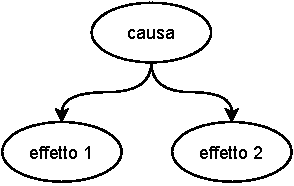
\includegraphics[scale = 0.9]{img/b.pdf}
\end{figure}
\begin{esempio}
  Vediamo un esempio:
  \[P(carie|mal\_di\_denti\land incastro)=\alpha P(|mal\_di\_denti\land
    incastro|carie)P(carie)\]
  \[=\alpha P(|mal\_di\_denti|carie)P(incastro|carie)P(carie)\]
\end{esempio}
\textbf{Ulteriori esempi su slide}.\\
\textit{Le probabilità congiunte le posso rappresentare in una tabella.}\\
Le \textbf{reti Bayesiane} sfruttano grafi diretti aciclici per rappresentare le
assunzioni di indipendenza condizionale tra variabili in modo chiaro ed
efficiente. Un arco diretto tra $A$ e $B$ rappresenta una relazione di
causalità: $A$ influenza $B$. Si ha quindi che ``pattern'' di ragionamenti sono
un cammino tra un nodo e un altro.\\
Si passa da $O(2^n)$ a $O(n)$, per $n$ numero di effetti.
\begin{definizione}
  Si ha che l'evento $A$ è condizionalmente indipendente dall'evento $B$ se,
  dato l'evento $C$:
  \[P(A|B,C)=P(A|C)\]
  ovvero la conoscenza di $B$ non porta a nessuna ulteriore variazione della
  probabilità di $A$ rispetto a quella dell'avverarsi di $C$. \\
  Dall'indipendenza di $A$ e $B$ dato $C$ si ha che:
  \[P(A,B|C)=P(A|C)P(B|C)=P(A,B|C)\]
  Se $C$ è un insieme vuoto ho, non avendo correlazione:
  \[P(A,B)=P(A)P(B)\]
\end{definizione}
Le reti Bayesiane quindi analizzano le cause dirette e indirette permettendo di
rappresentare in modo efficiente la distribuzione congiunta di probabilità,
tramite dipendenza e indipendenza condizionale.\\
L'inferenza basata su enumerazione è in $O(d^n)$ sia in spazio che tempo con:
\begin{itemize}
  \item $d$ massima cardinalità del supporto (se binario $d=2$)
  \item $n$ numero di variabili
\end{itemize}
è questo non va bene.\\
Una distribuzione congiunta può essere rappresentata come produttoria di $n$
valori di probabilità di \textbf{eventi indipendenti}, passando da un arrivando
a $O(n)$, avendo:
\[P(C_1,\ldots C_n)=P(C_1)\cdots \ldots P(C_n)\]
Rappresentando quindi, tramite l'indipendenza delle variabili, in modo compatto
una distribuzione congiunta. \\
Nel mondo reale però non si ha indipendenza assoluta tra le variabili e spesso
anche il gran numero di variabili rende difficile la specifica di una
distribuzione congiunta. \\
Si usa quindi l'indipendenza condizionale, sfruttando le variabili
condizionalmente indipendenti. \\
Per scrivere la definizione congiunta usiamo la \textbf{chain rule}.
Dato $P(X,Y,Z)$ si ha che, avendo $X$ e $Y$ indipendenti:
\[P(X,Y,Z)=P(X|Y,Z)P(Y,Z)=P(Z|Y,Z)P(Y|Z)P(Z)=P(X|Z)P(Y|Z)P(Z)\]
riducendo quindi il numero di valori di probabilità necessari al conto.\\
Le asserzioni di indipendenza condizionate si basano sul dominio in analisi e
consente di limitare le complessità del modello. Il caso in cui tutte le
variabili sono indipendenti ho la fattorizzazione delle probabilità delle
singole variabili ed è un caso specifico di questo discorso.\\
Ricordando che per Bayes:
\[P(Y|X)=\frac{P(X|Y)P(Y)}{P(X)}=\alpha P(X|Y)P(Y)\]
calcolando la probabilità della causa data la conoscenza dello stato degli
effetti. Quindi, avendo $X$ e $Y$ indipendenti:
\[P(X|Y,Z)=\alpha P(X,Y|Z)P(Z)=\alpha P(X|Z)P(Y|Z)P(Z)\]
Avendo graficamente $P(X,Y,Z)=\alpha P(X|Z)P(Y|Z)P(Z)$:
\begin{figure}[H]
  \centering
  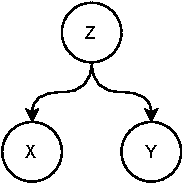
\includegraphics[scale = 0.9]{img/b2.pdf}
\end{figure}
Possiamo quindi parlare meglio delle \textbf{reti Bayesiane}, spesso indicata
con:
\begin{itemize}
  \item \textbf{Bayesian Belief Network, BBN}
  \item \textbf{Probabilistic Network, PN}
  \item \textbf{Causal Network, CN}
\end{itemize}
Tali reti appartengono alla classe dei \textbf{modelli
  grafico-probabilistici}.\\ 
\begin{definizione}
  Una \textbf{rete Bayesiana} è un grafo cui nodi sono annotati da una
  informazione quantitativa, tramite tabelle di probabilità condizionata, e i
  cui archi definiscono dipendenza e indipendenza tra le variabili dei nodi. Si
  hanno solo archi orientati. Se $X$ è causa diretta di $Y$ ho un arco tra $X$ e
  $Y$. $X$ è detto genitore e $Y$ figlio. Le variabili possono essere sia
  continue che discrete.\\
  La topologia della rete e le probabilità condizionate dei nodi dati genitori
  sono sufficienti a specificare (implicitamente) la distribuzione congiunta di
  tutte le variabili.\\
  Uno o più nodi isolati segnalano indipendenza assoluta. Due figli di uno
  stesso genitore segnalano che sono condizionalmente
  indipendenti. Nell'immagine $X$ e $Y$ sono condizionalmente indipendenti, $W$
  è indipendente dalle altre 3 variabili, $Z$ è causa diretta di $X$ e $Y$
  mentre tra queste ultime non esiste una relazione diretta di causalità:
  \begin{figure}[H]
    \centering
    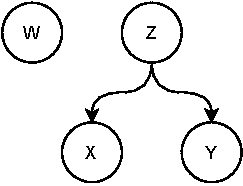
\includegraphics[scale = 0.9]{img/b3.pdf}
  \end{figure}
  Tale grafo non contiene cicli e quindi si parla di \textbf{Directed Acyclic
    Graph (\textit{DAG})}, non essendo possibile che una variabile causi se
  stessa. 
\end{definizione}
Come detto la componente quantitativa è costruita da un insieme di tabella di
probabilità condizionale. Ogni nodo ha associata quindi una \textit{Conditioned
  Probability Table (\textit{CPT})} che traduce l'impatto dei genitori sulla
variabile stessa.\\
\textbf{Su slide esempio esteso.}\\
Ricapitolando:
\begin{itemize}
  \item ogni nodo ha CPT
  \item ogni riga della CPT somma ad uno (e se ho un solo valore non scrivo sia
  il vero che il falso visto che posso fare $1-$)
  \item la CPT di una variabile booleana con $K$ variabili genitori contiene
  $2^K$ valori che possono essere specificati indipendentemente
  \item una variabile senza genitori ha una sola riga con i valori di
  probabilità a priori per ogni possibile valore che la variabile può assumere 
\end{itemize}
Possiamo dire che si hanno due chiavi di lettura dal punto di vista della
semantica, semanticamente equivalenti: 
\begin{itemize}
  \item la rete rappresenta una \textbf{distribuzione congiunta di
    probabilità}. Questa 
  lettura è utile per progettare e implementare procedure di inferenza. Per
  questa lettura dice che ogni rete costituisce una descrizione completa del
  dominio che rappresenta e pertanto ogni elemento della distribuzione di
  probabilità congiunta può essere calcolato a partire dall’informazione
  contenuta nella rete. Un generico elemento della distribuzione di probabilità
  congiunta è associato ad una realizzazione congiunta delle variabili (nodi)
  presenti nella rete:
  \[P(X_1=x_1\land\cdots\land X_n=x_n)=P(x_1,\ldots
    ,x_n)=\prod_{i=1}^nP(x_i|parents(X_i))\]
  che è detta \textbf{formula di fattorizzazione}.\\
  Avendo che con le maiuscole abbiamo le variabili (anche per $Parents$) e con
  le minuscole le realizzazioni (anche per $parents$). Si ha quindi che ogni
  elemento della distribuzione congiunta è rappresentato come prodotto di
  opportune componenti delle CPT che costituiscono quindi una rappresentazione
  decomposta della distribuzione di probabilità congiunta. Per questa
  rappresentazione posso usare le reti per rispondere a qualsiasi query relative
  al dominio che descrive tramite marginalizzazioni.\\
  \textbf{Esempio su slide}.
  
  \item la rete codifica un \textbf{insieme di relazioni di indipendenza
    condizionale}. Questa lettura è utile per costruire un modello di rete
  Bayesiana.
\end{itemize}
Sfrutto la formula di fattorizzazione per determinate la
componente topologica della rete. Si ricorda che per la \textbf{cchin rule}:
\small{\[P\left(x_{1}, \ldots, x_{n}\right)=P\left(x_{n} \mid x_{n-1}, \ldots,
      x_{1}\right) \cdot P\left(x_{n-1} \mid x_{n-2}, \ldots, x_{1}\right) \cdot
    \ldots \cdot P\left(x_{2} \mid x_{1}\right) \cdot
    P\left(x_{1}\right)\]\[
    =\prod_{i=1}^n P\left(x_{i} \mid x_{n-1}, \ldots,
      x_{1}\right)\]}
Noto che tale formula è confrontabile con la formula di fattorizzazione e ho
che, a patto che $Parents(X_1)\subseteq \{x_{i-1},\ldots,x_1\}$:
\[\mathbf{P}\left(x_{i} \mid x_{i-1}, \ldots,
    x_{1}\right)=\mathbf{P}\left(x_{i} \mid \text { parents
    }\left(X_{i}\right)\right)\] 
Quindi una Rete Bayesiana rappresenta correttamente un dominio solo a
condizione che ogni nodo risulti condizionalmente indipendente dai suoi
predecessori, per un dato ordinamento, dati i suoi genitori. Pertanto, per
costruire una Rete Bayesiana che abbia la corretta struttura del dominio da
modellare è necessario scegliere, per ogni nodo, i nodi genitore in modo che
tale proprietà risulti verificata. Quindi i genitori di $X_i$ devono essere
scelti da $\{X_1,\ldots,X_{i-1}\}$.\\
Si ha quindi la seguente procedura di costruzione incrementale della
componente topologica;
\begin{enumerate}
  \item Si seleziona un insieme di variabili $\{X_1,\ldots, X_n\}$ per
  descrivere il modello
  \item scelgo un ordinamento per le variabili $\{X_{(1)},\ldots,
  X_{(n)}\}$. Con un ordinamento sbagliato arrivo a definire reti sbagliate o
  reti più complesse del necessario, magari con informazioni ridondanti
  \item inizializzo i nodi aggiunti alla rate partendo da $i=1$
  \item si seleziona la variabile $X_{(i)}$ alla rete, si pone
  $Parents(X_{(i)})$ uguale all’insieme minimale di nodi, attualmente
  appartenenti alla rete ${X_{(1)},\ldots, X_{(i-1)}}$, che soddisfa la
  proprietà di indipendenza condizionale:
  \[\mathbf{P}\left(X_{(i)} \mid X_{(i-1)}, \ldots,
      X\right)=\mathbf{P}\left(X_{(i)} \mid\right. \text { Parents
    }\left(X_{(i)}\right)\]
  per poi calcolare la CPT di $X_{(i)}$
  \item tengo conto del nodo aggiunto nel conto totale dei nodi e faccio
  i++. Se ho finito le variabili termino altrimenti torno a 4)
\end{enumerate}
Una rete è più compatta, solitamente, dell'intera distribuzione di probabilità
congiunta e tale compattezza è un esempio della proprietà dei \textbf{sistemi
  strutturati localmente o sparsi}, dove ogni sotto-componente interagisce solo
con un numero limitato di 
altre componenti, indipendentemente dal numero totale di componenti del
sistema. La strutturazione locale normalmente ha crescita lineare e non
esponenziale (mediamente con una rete Bayesiana è ragionevole pensare che ogni
variabile sia influenzata da al massimo $k$, con $k$ costante, variabili).\\  
Nel caso in cui si consideri una Rete Bayesiana costituita da $n$ variabili
(nodi) booleane. Si ha che la quantità di informazione per specificare una CPT è
limitata superiormente da $2^k$ per cui la rete completa richiede $n\cdot 2^k$
cifre contro i $2^n$ dell'intera distribuzione di probabilità congiunta.\\
Si hanno quindi vari tipi di rete, relativi a situazioni diametralmente opposte:
\begin{itemize}
  \item \textbf{rete completamente connessa (\textit{fully connected network})},
  dove ogni variabile può essere potenzialmente influenzata da tutte le altre e
  quindi specificare una CPT richiede le stesse informazioni della distribuzione
  congiunta
  \item \textbf{rete con relazioni di causalità tenui} dove se aggiungo delle
  relazioni, degli archi aumento la complessità della rete (???). Si valuta il
  guagno in accuratezza contro quelle in complessità
\end{itemize}
Anche in un dominio strutturato localmente la costruzione di una Rete Bayesiana
non è semplice, volendo un numero limitato di influenze per ogni variabile e che
la topologia della rete rifletta le relazioni di influenza diretta. La procedura
di costruzione di una Rete Bayesiana funziona in modo tale che quando si giunge
ad aggiungere un nodo, i nodi candidati ad essere suoi genitori, ovvero i nodi
che lo influenzano direttamente o indirettamente, siano già stati aggiunti alla
corrente struttura della rete. Il corretto ordine comporta che si devono prima
stabilire le cause radice per poi aggiungere quelle variabili che da loro
vengono influenzate, procedendo fino alle foglie che non sono causa di nulla. \\
lato \textbf{semantica topologica} abbiamo due specificazioni equivalenti:
\begin{itemize}
  \item un nodo è condizionalmente indipendente dai suoi non-discendenti dati
  suoi genitori
  \item un nodo è condizionalmente indipendente da tutti i nodi restanti della
  rete, data la conoscenza dello stato dei suoi genitori, dei suoi figli e dei
  genitori dei suoi figli. Tale insieme di nodi è detto \textbf{Markov Blanket}
\end{itemize}
Vediamo come capire se in una rete Bayesiana due variabili sono condizionalmente
indipendenti.
\begin{definizione}
  Definiamo che $X$ e $X$ sono \textbf{d-separati} da un insieme $E$ di
  variabili con evidenza (ovvero osservazioni) sse ogni cammino non orientato da
  $X$ a $Z$ è \textbf{bloccato} ovvero sse:
  \begin{itemize}
    \item lungo il cammino si ha una variabile $V\in E$ (quindi di cui conosco
    il valore) e gli archi che
    collegano $V$ al cammino sono solo \textbf{tail to tail} (ovvero da $V$
    escono i 
    due archi: $\to V\gets$) e quindi il cammino è bloccato da $V$
    \item lungo il cammino si ha una variabile $V\in E$ (quindi di cui conosco
    il valore) e gli archi che
    collegano $V$ al cammino sono solo \textbf{tail to head} (ovvero un arco
    entra in 
    $V$ ed uno esce: $\to V\to$) e quindi il cammino è bloccato da $V$
    \item lungo il cammino si ha una variabile $V\not\in E$ (quindi di cui NON
    conosco il valore) tale che nessuno dei
    suoi discenti appartiene all'insieme $E$ e gli archi che
    collegano $V$ al cammino sono solo \textbf{head to head}
  \end{itemize}
\end{definizione}
\textbf{Esempi su slide}.\\
\begin{teorema}[teorema di Verma e Pearl]
  Se in una rete Bayesiana un insieme $E$ di variabili con evidenza d-separa $X$
  e $Y$ allora $X$ e $Y$ sono indipendenti.
\end{teorema}
La d-separazione si calcola in tempo lineare avendo quindi un algoritmo
efficiente per inferire automaticamente se apprendere il valore di una variabile
può fornire informazioni aggiuntivi su altre variabili date le informazioni a
disposizione quindi può essere utile per capire se apprendere il valore di una
delle due variabili può aiutarci ad avere informazione aggiuntiva rispetto
all’altra.\\ 
Si hanno algoritmi di propagazione dell'informazione che portano a calcolare la
distribuzione di probabilità, incondizionata o marginale, su ogni nodo. Tale
distribuzione è detta anche \textbf{belief function} del nodo. \\
L'algoritmo di propagazione aggiorna le belief di ogni nodo della rete ogni
volta che si ha una nuova evidenza (???).\\
\textbf{Esempi su slide. Su elearning file sulla \textit{Moralizzazione},
  argomento extra}.\\
Anche avendo massimo $k$ genitori per ogni variabile si ha che servono $O(2^k)$
parametri per ogni CPT.\\
Si ha una distribuzione canonica per rappresentare pattern standard per avere un
numero limitato di parametri per compilare la CPT. Uno di questi pattern è detto
\textbf{modi deterministici}. Un nodo deterministico ha che il suo valore è
determinato unicamente da quello dei genitori, senza incertezza, avendo quindi
una relazione ad esempio logica (\textit{and, or,} etc$\ldots$) o numerica
(\textit{max, min, }etc$\ldots$). Ovviamente non tutta la rete è fatta da questi
nodi altrimenti non userei una rete Bayesiana ma in una rete complessa si
possono avere tali pattern. Tramite tali relazioni calcolo direttamente i valori
delle CPT.\\
Un altro pattern, in presenza di incertezza, è quello \textbf{noisy logical
  relationship}, con generalizzazioni degli operatori logici. Un esempio è il
\textbf{noisy-OR}, che introduce incertezza circa la capacità di causare $\top$
nella variabile figlio da parte del nodo genitore. Si ha che la relazione di
causalità tra genitore e figlio potrebbe essere inibita. Con noisy-OR si hanno due
ipotesi:
\begin{itemize}
  \item tutte le possibili cause sono note (eventualmente si possono aggiungere
  \textit{leak node}, un nodo fittizio per rendere esaustive la cause)
  \item l'inibizione di un genitore è indipendente da quella di altri genitori
  per il nodo considerato
\end{itemize}
L'inibizione è legata ad una certa probabilità, dette \textit{probabilità di
  inibizione}, ovvero \textbf{noise parameters}.\\
La probabilità di un evento viene ottenuta tramite il prodotto delle probabilità
di inibizione di ogni nodo genitore. Quindi per certe combinazioni di or non ho
il valore preciso ma una certa probabilità. Se esattamente un genitore è $\top$
allora il figlio è $\top$ con probabilità pari al noise parameter di tale
genitore. Se nessun genitore è nello stato $\top$ allora certamente il figlio è
nello stato $\bot$. Negli
altri casi appunto moltiplico i noisy parameter dei genitori con valore
$\top$. Ho quindi limitato il numero di parametri. Quindi se una variabile
dipende da $k$ genitori di norma ho la noisy-OR con $O(k)$ parametri e non
$O(2^k)$, per descrivere l'intera distribuzione di probabilità congiunta.\\
\textbf{Esempi su slide}.\\
Potrei avere \textbf{reti con nodi continui} e potendo assumere un numero
infinito di valori si rende impossibile specificare esplicitamente i valori della
distribuzione condizionale e di quella a priori. Si procede quindi
\textbf{discetizzando} i valori in un numero finito di intervalli, perdendo
comunque di informazione, soprattutto con grandi CPT. Una alternativa sono le
\textbf{funzioni di densità di probabilità}, trascritte un numero finito e,
solitamente, contenuto di parametri.\\
Un esempio di tale funzione è la \textbf{gaussiana univariata}:
\[N(\mu,\sigma^2)\]
che ha due parametri: \textit{media} e \textit{varianza}.\\
Una rete con nodi discreti e continui insieme è detta \textbf{rete Bayesiana
  ibrida} e per la sua definizione servono due tipi di distribuzione:
\begin{itemize}
  \item la distribuzione condizionale di una variabile continua dati i genitori
  discreti o continui
  \item la distribuzione condizionale di una variabile discreta dati i genitori
  continui 
\end{itemize}
Usando quindi questa \textit{gaussiana lineare} (comoda perché facendo
operazioni tra gaussiane si ottiene comunque una gaussiana) perché il nodo
figlio è 
distribuito secondo una distribuzione gaussiana la cui media $\mu$ varia
linearmente con il valore del genitore mentre la deviazione standard $\sigma$ è
fissata. In pratica si fa una sorta di regressione lineare con rumore
gaussiano. Si ha che la gaussiana lineare ha 2 proprietà:
\begin{enumerate}
  \item una rete che contiene solo nodi continui con distribuzione Gaussiana
  Lineare ha una 
  distribuzione di probabilità congiunta \textbf{Gaussiana multivariata}
  \item una rete che contiene nodi continui con distribuzione Gaussiana Lineare
  e nodi discreti, 
  nessuno dei quali sia figlio di nodi continui, definisce una distribuzione
  Gaussiana Condizionale 
  per ogni assegnamento di valori per le variabili discrete; la distribuzione
  sulle variabili continue 
  è \textbf{Gaussiana multivariata}
\end{enumerate}
Avendo una cosa del tipo $P(c|r,s=\top)$ si avrebbe:
\[N(a_\top\cdot r+b_\top, \sigma_\top^2)(c)=\frac{1}{\sqrt{2\pi}\cdot
    \sigma_\top}e^{-\frac{1}{2}\left(\frac{c-(a_\top\cdot
        r+b_\top)}{\sigma_\top}\right)^2}\]
dovendo poi fare un discorso analogo per $\bot$. Si ha che $a$ e $b$ sono il
legame con la regressione lineare.\\
\textbf{Esempio su slide}.\\
Anche usando modelli semplici si possono ottenere distribuzioni flessibili e
interessanti. \\
Passiamo ora alla \textbf{distribuzione associata a variabili discrete con
  genitori continui}, tramite una \textbf{funzione a soglia soft}. \\
Un modo di ottenere soglie soft è usare l'integrale della normale standard:
\[\phi(x)=\int_{-\infty}^x N(0,1)(x)\dd{x}\]
usando la distribuzione \textbf{probit}:
\[P(X|Y=c)\phi(\frac{-c+\mu}{\sigma})\]
il che significa che la soglia di costo si verifica intorno al valore μ, lo
spessore della regione soglia è 
proporzionale al valore $\sigma$, e la probabilità di acquistare diminuisce
all’aumentare del costo. \\
In alternativa si ha la funzione \textbf{probit}, che utilizza la
\textbf{funzione sigmoid} per ottenere una soglia soft:
\[P(X|Y=c)\phi(\frac{1}{1+e^{-2\cdot\frac{-c+\mu}{\sigma}}})\]
\subsection{Inferenza nelle Reti Bayesiana}
Lo scopo di un modello probabilistico è quello di ottenere la distribuzione a
posteriori, per un certo insieme di variabili query, in presenza di un evento,
ovvero un assegnamento congiunto di valori ad un insieme di variabili con
evidenza. Sono dati:
\begin{itemize}
  \item $X$ variabile query
  \item $E$ insieme delle evidenze $E_i$
  \item $e$ evento specifico
  \item $Y$ insieme variabili non evidenziate $Y_i$
\end{itemize}
L'insieme completo delle variabili è:
\[\mathbf{X}=\{X\}\cup E\cup Y\]
e si hanno query del tipo:
\[P(X|E=e)\]
Dato un modello di rete Bayesiana si hanno 4 tipologie di inerenza;
\begin{itemize}
  \item \textbf{diagnostica}, avendo l'effetto si vuole capire la causa
  \item \textbf{causale}, avendo la causa voglio stimare la probabilità degli
  effetti 
  \item \textbf{intercausale}, avendo una causa, capire
  la probabilità un'altra causa di un effetto comune
  \item \textbf{mista}, avendo sia diagnostica che causale o sia diagnostica che
  intercausale 
\end{itemize}
\begin{figure}
  \centering
  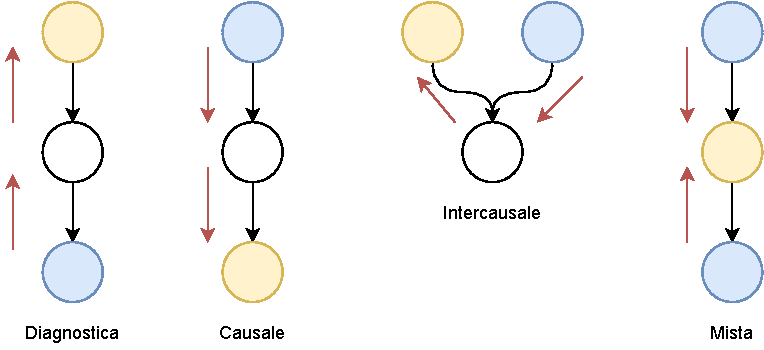
\includegraphics[scale = 0.8]{img/inf.pdf}
  \caption{Tipi di inferenza, in blu l'evidenza e in giallo la variabile $X$}
\end{figure}
Avere osservato che uno degli eventi fa divenire meno probabile che un altro si
sia verificato è il meccanismo di
\textbf{explaining away}.\\
Con una rete Bayesiana quindi posso cercare:
\begin{itemize}
  \item probabilità condizionata $P(X|e)$
  \item quale valore massimizza $P(X|e)$, cercando la massima probabilità a
  posteriori
  \item quale è la distribuzione di probabilità di $X$ dato $e$ (che è il caso
  generale) 
\end{itemize}
Ogni distribuzione condizionale può essere ottenuta
tramite un procedimento di somma di opportuni elementi dell’intera distribuzione
di probabilità congiunta 
(marginalizzazione). Si ha quindi che:
\[P(X|E=e)=\alpha\cdot P(X,E=e)=\alpha\cdot \sum_y P(X,E=e, Y=y)\]
e con la regola di fattorizzazione delle reti Bayesiane:
\[P(x_1,\ldots,x_n)=\prod_{i=1}^nP(x_i|parents(X_i))\]
e quindi $P(X,E=e, Y=y)$ nella distribuzione congiunta, possono essere scritti
sotto 
forma di prodotti di probabilità condizionali della rete.
In definitiva concludiamo che:
\begin{center}
  \textit{Ad una query è possibile rispondere utilizzando una Rete Bayesiana
    tramite la computazione di 
    somme di prodotti di probabilità condizionali della rete}
\end{center}
Vedremo sia algoritmi esatti che approssimati, tramite campionamento, per
l'inferenza.\\
\section{Inferenza esatta}
Per fare inferenza esatta sfruttiamo l'equazione:
\[P(X|E=e)=\alpha\cdot P(X,E=e)=\alpha\cdot \sum_y P(X,E=e, Y=y)\]
sfruttando la fattorizzazione, che fornisce un'espressione in termini di CPT per
effettuare il calcolo.\\
\textbf{Esempio su slide}.\\
Nel caso peggiore, dovendo marginalizzare tutte le variabili, ho un algoritmo,
per una rete di $n$ variabili booleane, di complessità:
\[O(n\cdot 2^n)\]
ma a seconda dei casi posso effettuare delle ottimizzazioni, estraendo elementi
costanti dalle sommatorie generate usando la chain rule (\textbf{guardare sempre
  esempio su slide}).\\
Per ogni sommatoria che si crea poi eseguo l'\textbf{algoritmo di enumerazione},
vedendo l'algoritmo come una sorta di struttura ad albero. Si richiede quindi di
iterare su tutte le possibili realizzazioni congiunte delle variabili
coinvolte. \\
Con queste ottimizzazioni si arriva a:
\[O(2^n)\]
Un miglioramento comunque non sufficiente.\\
Studiando l'albero di computazione si notano ripetizioni di computazione quando
si effettua l'algoritmo di enumerazione, che consiste nella valutazione
ricorsiva di tale albero. Si memorizzano quindi le operazioni già fatte per non
doverle ripetere, ad esempio tramite \textbf{l'algoritmo di eliminazione
  variabili}. Questo algoritmo valuta da destra a sinistra, ovvero bottom-up, le
espressioni e memorizza i risultati intermedi mentre la marginalizzazione viene
effettuata solo per le porzioni di espressione che dipendono dalla variabile
stessa. \\
Tale algoritmo si basa sul fatto che ogni variabile che non sia predecessore di
una variabile in studio o di una variabile con evidenza è irrilevante nello
studio 
della query. Si rimuovono quindi dall'albero le variabili inutili, ovvero quelle
oggetto della query e quelle con evidenza. \\
L'ordine di eliminazione influisce sulla complessità temporale complessiva. Con
reti molto complesse magari non binarie, il problema resta di elevata
complessità e non ci si può aspettare di poter fare inferenza esatta su tali
reti. \\
Con le reti Bayesiane si nota che è possibile fare, a seconda della query,
calcolo parallelo. Si ragiona comunque solitamente per campionamenti, generando
configurazioni possibili della rete tramite le distribuzioni della CPT e
calcolano la frequenza in cui una certa variabile assume un certo valore date le
evidenze. Per farlo bisogna generare numeri pseudocasuali.
\section{Numeri Pseudocasuali}
Innanzitutto su un numero singolo non possiamo dire nulla in merito alla sua
casualità. Se uno dice 3 non posso inferire nulla sulla sua casualità.\\
Una lista di numeri può apparire casuale ma potrebbe non esserlo.
\begin{definizione}
  una \textbf{sequenza di numeri pseudo casuali} è una sequenza di realizzazioni
  di 
  variabili aleatorie indipendenti e identicamente distribuite.\\
  Tali numeri sembrano impredicibili e senza regolarità. ``Sembrano'' perché
  comunque dietro si ha un meccanismo di calcolo.
\end{definizione}
Il lancio dei dadi è un metodo manuale valido, completamente causale al più di
trucchi, ma richiede troppo tempo. Esistono anche 
device specifici per farlo ma si hanno altri problemi, si preferisce quindi un
calcolatore che genera le stesse sequenze, in modo pseudocasuale.\\
Serve un \textbf{seme di generazione}, avendo che con un seme genero sempre la
stessa sequenza e questo è importante per poter valutare due sistemi in base
agli stessi scenari, rigenerando sempre la stessa sequenza. Questa è la
\textbf{proprietà di riproducibilità}.\\
I numeri causali generati devono avere una serie di proprietà statistiche,
devono sembrare impredicibili ma:
\begin{itemize}
  \item la distribuzione deve essere, o perlomeno simulare, una distribuzione
  uniforme, 
  verificabile all'aumentare dei 
  numeri generati tramite il calcolo della media (che deve essere a metà del
  range nel quale si hanno numeri generati, se range $[0,9]$ voglio media $4.5$)
  \item devo avere indipendenza statistica
  \item devo avere riproducibilità di valori
  \item non devo avere ripetitività su un prefissato periodo abbastanza lungo,
  se avessi periodi troppo brevi potrei fare predizione
\end{itemize}
Il seme, se non specificato, viene scelto via hardware, tipo il clock attuale
della cpu etc$\ldots$\\
La routine che genera numeri pseudocasuali di default genera una distribuzione
uniforme su $[0,1]$ deve:
\begin{itemize}
  \item essere veloce
  \item avere periodi di ripetizioni lunghe
  \item non presentare lunghi gap tra la generazione di due numeri, nella
  discretizzazione di variabili continue, avendo uniformità
  \item essere replicabile
 \item generare sequenze con proprietà statistiche simili a quelle reali
\end{itemize}
Uno dei primi algoritmi è stato quello di Von Neumann, detto \textbf{middle
  square}, che genera un numero con 10 cifre. Si parte da un numero, il seed, si
eleva al 
quadrato e si prendono le 10 cifre centrali, che saranno il prossimo numero. In
realtà è molto pseudocasuale avendo che ogni numero dipende dal precedente ma
sembra causale e si hanno casi di numeri che comportano facilmente la
riconoscibilità di tale pattern o che addirittura generano un loop, tornando al
seme dopo poche generazioni.  \\
Nel tempo si sono quindi di studiati vari parametri iniziali dell'algoritmo. \\
Un primo metodo, detto \textbf{moltiplicative congruential method
  (\textit{MCM})}, prevede: 
\[x_n=a\cdot x_{n-1},\,\,\,0\leq x_n\leq m\]
con $a$ e $m$ interi scelti e un $x_0$ seed. La scelta di $m$ deve essere tale
per avere cicli molto ampi e quindi $m$ è solitamente molto grande, nonché primo
(cosa capita empiristicamente). Sono state studiate varie combinazioni di $m$ e
$a$, come $m=2^{31}-1$ e $a=7^5$ o $m=2^{35}-31$ e $a=5^5$. Siu ha che $m$ deve
portare ad avere pochi gap.\\
Si ha poi il \textbf{linear conrguential method (\textit{LCM})}, che prevede:
\[x_n=(a\cdot x_{n-1}+c)\bmod m\]
con anche $c$ scelto opportunamente. Si ha che:
\begin{itemize}
  \item $a,c\geq 0$
  \item $m>x_0,c,a$
\end{itemize}
Però ci servono variabili aleatorie uniformi in $[0,1]$ quindi devo fare, per
LCM: 
\[u_n=\frac{x_n}{m}\]
Con LCM si ha ciclo pari a $m$ e si generano numeri discretizzati e quindi serve
un $m$ molto grande (ma anche qui si hanno scelte di parametri ``sfortunate'',
che comportano cicli brevi).\\
Un ciclo normalmente deve tendere al numero intero massimo rappresentabile, ma
dipende dai casi.\\
Aumentare $m$ riduce periodicità e generazione di numeri razionali. Solitamente
$m\geq 10^9$, per ottenere un sottoinsieme denso in $[0,1]$. Solitamente $m$ è
quindi il massimo intero rappresentabile.\\
Il \textbf{generatore di Learmouth-Lewis} prevede:
\begin{itemize}
  \item $c=0$
  \item $a=75$
  \item $m=2^{31}-1$
\end{itemize}
Che è uno dei più usati ma si hanno molti altri generatori.\\
A partire dai numeri tra 0 e 1 posso passare a distribuzioni arbitrarie.\\
\subsection{Generazione di Distribuzione Generica}
Partiamo ora da una sequenza di numeri pseudocasuali $U(0,1)$. Si hanno varie
tecniche per la generazione di una distribuzione generica:
\begin{itemize}
  \item \textbf{tecnica di trasformazione inversa}
  \item \textbf{metodo di accettazione rifiuto}
  \item \textbf{metodo di composizione}
\end{itemize}
In generale si vuole utilizzare poche volta la routine di generazione di numeri
random. \\
Ricordiamo due concetti:
\begin{itemize}
  \item \textbf{funzione di densità} che prevede:
  \[P(x=x_1)=0\]
  e:
  \[P(x_1-\varepsilon\leq X\leq
    x_1+\varepsilon)=\int_{x_1-\varepsilon}^{x_1+\varepsilon} f_X(x)\dd{x}\]
  \item \textbf{distribuzione cumulativa}, che prevede;
  \[F_X(x)=p(X\leq x)=\int_{-\infty}^x f_X(y)\dd{y}\]
\end{itemize}
\subsubsection{Trasformazione Inversa}
Vogliamo ora generare una variabile aleatoria $X$ con funzione di densità di
probabilità:
\[f_X(x)\]
Si hanno quindi vari step:
\begin{enumerate}
  \item si calcola la funzione di distribuzione di probabilità o funzione
  cumulativa di probabilità:
  \[F_X(x)=\int_{-\infty}^Xf_X(\tau)\dd{\tau}\]
  che, qualora sia possibile calcolarla in forma chiusa, è continua, monotona,
  crescente e compresa tra 0 e 1, avendo $F_X(x)=p(X\leq x)$
  \item si pone:
  \[u=F_X(x)\]
  con $u$ numero random $(u-U(0,1)$
  \item si risolve:
  \[X=F_X^{-1}(u)\]
  ottenendo che la variabile aleatoria $X$ è distribuita secondo $f_X(x)(X\sim
  f_X(x))$ 
\end{enumerate}
Vediamo quindi qualche caso particolare.\\
Supponiamo di voler costruire una successione di numeri pseudocasuali come
osservazioni dalla \textbf{distribuzione esponenziale} ovvero con funzione di
distribuzione:
\[F(x)=1-e^{\lambda\cdot x}\]
Ho quindi:
\[U=F(x)=1-e^{\lambda\cdot x}\implies 1-U=e^{\lambda\cdot x}\]
e quindi:
\[\ln(1-U)=\ln(e^{\lambda\cdot x})\implies \ln(1-U)=-\lambda\cdot x\]
e quindi:
\[x=-\frac{\ln(1-U)}{\lambda}\]
e quindi:
\[x=F^{-1}(U)=-\frac{\ln(1-U)}{\lambda}\]
e se $U$ è una variabile aleatoria con distribuzione uniforme su $[0,1)$ ho che
$x$ è una variabile aleatoria con distribuzione esponenziale con media
$\frac{1}{\lambda}$. Da una successione di numeri pseudocasuali uniformi ottengo
una successione di numeri pseudocasuali con distribuzione esponenziale. \\
Inoltre se $U$ è in [0,1) lo è anche $1-U$ e quindi sostituisco $(1-U)$ con $U$
nella formula, anche se questo cambiamento potrebbe indurre un cambiamento nella
correlazione delle variabili $X$ generate. \\
Quindi la routine di generazione di $X$ con funzione di densità di probabilità
esponenziale chiama una sola volta per ogni $X$ la routine di generazione di
numeri casuali $R$. Si ha, per la routine di $X$, quindi lo stesso ciclo di tale
routine $R$ e gap crescenti per 
$X$ crescente. Se la routine è replicabile lo è anche quella per $X$. Se la
routine di generazione è ideale lo è anche quella di $X$.\\
Posso estendere il metodo a distribuzioni discrete, con $X$ \textbf{variabile
  aleatoria discreta}. \\
Suppongo $X$ con valori $x_1,x_2,\ldots$ con:
\[x_1<x_2<\ldots\]
Data $U$ variabile uniformemente distribuita in $[0,1)$ si ha che:
\[X(U)=\max\{x_i|\,U\in[F(x_i-1)-F(x_i)]\}\]
Si ha quindi, avendo $P(X=i)=p_i$:
\begin{itemize}
  \item \textbf{funzione di densità}:
  \[\sum_{i=\infty}^\infty P(X=i)=1\]
  \item \textbf{Distribuzione cumulativa}:
  \[F_X(x)=P(X\leq x)=\sum_{i=-\infty}^xP(X=i)\]
\end{itemize}
In generale si ha che:
\[P(X=x_j)=p_j,\,\,\,j=0,1,\ldots, n\]
con:
\[\sum_{j=0}^np_j=1\]
e ho:
\begin{itemize}
  \item $x_0$ se $u\leq p_0$
  \item $x_1$ se $p_0\leq \leq p_0+p_1$
  \item $\cdots$
  \item $x_j$ se $\sum_{i=0}^{j-1} p_i\leq u\leq\sum_{i=0}^j$
  \item $\cdots$
\end{itemize}
In base a questo si possono avere procedure più efficienti di altre (???),
rendendo la ricerca di appartenenza dell'intervallo il più efficiente
possibile.\\
Ad esempio, volendo generare una distribuzione discreta uniforme con:
\begin{itemize}
  \item $X\varepsilon\{0,1,\ldots,n\}$ (???)
  \item $p_0=p_1=\cdots p_n=\frac{1}{n+1}$ 
\end{itemize}
Ottenendo:
\[X=\lfloor (n+1)\cdot u\rfloor\]
\subsection{Metodo Acceptance-Rejection}
Il metodo precedente si basava sul calcolo di $F^{-1}$ ma non sempre questo è
possibile in modo efficiente, a seconda della funzione. Si sono stati quindi
creati altri metodi, più generali, come il 
\textbf{metodo Acceptance-Rejection}, detto anche \textbf{metodo del rigetto}.\\
Suppongo una distribuzione definita su $[a,b]$. Suppongo di conoscere la densità
di probabilità della variabile aleatoria $X$ tale che $f_X(x)$ è su $[a,b]$ e la
sua immagine è definita sul codominio $[0,c]$. In pratica tale funzione è in un
rettangolo $[a,b]\times[0,c]$. Si genera quindi un numero in questo rettangolo e
se cade fuori dalla funzione lo rifiuto, altrimenti lo accetto.\\
Si generano due sequenze pseudocasuali uniformi tra $[0,1]$ e le chiamo $U_1$ e
$U_2$. Si generano quindi altre due sequenze uniformi ytramite:
\[
  \begin{cases}
    X=a+(b-a)\cdot U_1\\
    Y=c\cdot U_2
  \end{cases}
\]
rimappando $[0,1]$ in $[a,b]$ e in $[0,c]$. Quindi ad ogni $(U_1,U_2)$ si ha
$(X,Y)$ che è nel rettangolo. Se quest'ultima cade nell'area della funzione
viene accettata e in caso contrario rifiutata, provando una nuova coppia. La
sequenza di valori ottenuta segue quindi la distribuzione data dalla funzione.\\
Il metodo è più efficiente quando l'area della funzione copre quasi interamente
il rettangolo, avendo lo scarto di poche coppie. Si hanno quindi i seguenti
step per generare una variabile aleatoria $X$, con funzione di densità di
probabilità $f_X(x)$ su $[a,b]$:
\begin{itemize}
  \item si genera una variabile $R$ distribuita in modo uniforme su $[a,b]$,
  ovvero $U(a,b)$
  \item si accetta tale valore con probabilità pari a:
  \[\frac{F_X(R)}{\max F_X(x)}\]
  in quanto il rettangolo è ``aderente'' alla funzione e la $c$ tende a
  coincidere con il massimo della funzione. Tale numero è rifiutato con
  probabilità:
  \[1-\frac{F_X(R)}{\max F_X(x)}\]
\end{itemize}
Dove la funzione è ``bassa'' si scartano più valori.\\
La routine di generazione di tale variabile aleatoria $X$ quindi:
\begin{itemize}
  \item chiama due volte la routine che genera un numero random, una per $R$ e
  una per capire se accettare e rifiutare
  \item ciclo e gap dipendono dal prodotto tra questi due numeri casuali ed p
  replicabile se lo è la routine di generazione del numero casuale
  \item è da usare solo se non si hanno altri metodi
\end{itemize}
\section{Inferenza Approssimata}
Il poter generare numeri causali serve al campionamento. Se le reti hanno una
certa struttura posso usare l'inferenza esatta ma in generale è un problema
NP-hard. SI usa quindi solo su reti singolarmente connesse, dove si ha al più un
cammino orientato tra coppie di nodi. Tali reti sono dette \textbf{polytree} e
permettono complessità spaziale e temporale lineare nella dimensione della rete
(ovvero nel numero di elementi della CPT). Addirittura se il numero di genitori
di ogni nodo è limitato da una costante si ha tempo lineare nel numero di
nodi.\\
Per rispondere a query univariate posso usare la \textbf{eliminazione delle
  variabili}.\\
La computazione della probabilità a posteriori per tutte le variabili può essere
meno efficiente, ad esempio in un polytree si arriva a $O(n^2)$. Per restare in
$O(n)$ si usano algoritmi di clustering, dove si uniscono nodi per ottenere un
polytree, dove si può poi usare un metodo efficiente. Purtroppo anche gli
algoritmi di clustering presentano inferenze NP-hard, per la costruzione delle
CPT dei cluster.\\
Per reti multiplamente connesse si usano quindi algoritmi di inferenza
approssimata, tramite algoritmi \textbf{Monte Carlo}, la cui accuratezza dipende
dal numero di campioni generati.\\
Vedremo due metodi:
\begin{itemize}
  \item \textbf{direct sampling}
  \item \textbf{Markov chain sampling}
\end{itemize}
\subsection{Direct Sampling}
In primis bisogna generare campioni secondo una distribuzione di probabilità,
tramite generazione di numeri pseudocasuali, che è l'idea di base di ogni
algoritmo di campionamento. \\
Partiamo dl caso semplice, dove si ha una rete Bayesiana senza variabili con
evidenza. Si campiona quindi la rete, seguendo l'ordine topologico partendo
dalla radice e campionando le variabili. La scelta della distribuzione per il
campionamento è quella che risulta dal condizionamento sui valori del nodo
genitore. Tale algoritmo è detto \textbf{campiona-Priori}, che ha in input la
rete e genera/campiona le variabili della rete. Tali campioni simulano la
distribuzione congiunta della rete. Genero in pratica possibili configurazioni
della rete. \\
\textbf{Esempio su slide}.\\
L'algoritmo genera quindi campioni della distribuzione di probabilità congiunta
a priori. Chiamo:
\[S_{CP}(x_1,\ldots,x_n)\]
come la probabilità che uno specifico evento sia generato tramite l’algoritmo
Campiona-Priori. Sappiamo poi che:
\[S_{CP}(x_1,\ldots,x_n)=\prod_{i=1}^nP(x_i|parents(x_i))\]
in quanto ogni campione dipende solo dai genitori. Questo ricordiamo rappresenta
la probabilità dell'evento considerato secondo la distribuzione di probabilità
con giunta della rete, la fattorizzazione. Si ha quindi che:
\[S_{CP}(x_1,\ldots,x_n)=P(x_1,\ldots,x_n)\]
rendendo semplice rispondere alla query.\\
Le risposte, dati $N$ campioni, vengono date tramite conteggio dei campioni. SI
ha che:
\[N_{cp}(x_1,\ldots,x_n)\]
è la frequenza per l'evento $(x_1,\ldots x_n)$ negli $N$ campioni.\\
Ogni campione da un contributo paritario e ci si aspetta che la frequenza
convenga al valore atteso in accordo con la distribuzione da cui si estraggono
gli $N$ campioni:
\[\lim_{N\to\infty}\frac{N_{cp}(x_1,\ldots,x_n)}{N}
  =S_{CP}(x_1,\ldots,x_n)=P(x_1,\ldots,x_n)\]
Campionando in modo indipendente generiamo campioni che rappresentano la
distribuzione della rete, quindi all'aumentare di $N$ ci si aspetta che un
evento compaia con la giusta probabilità, anche se comunque è un ``tende'', per
cui si parla di inferenza approssimata.\\
Con $\approx$ si indica la probabilità stimata, che diviene esatta per
$N=\infty$. Tale stima è detta \textbf{consistente}, avendo, per $m\leq n$:
\[P(x_1,\ldots,x_m)=\frac{N_{PS}(x_1,\ldots,x_m)}{N}\]
La probabilità di un evento parzialmente specificato viene stimata come la
frazione dei casi compatibili con l’evento parzialmente specificato sul numero
di tutti i casi generati tramite campionamento. \\
Passiamo ora all'avere evidenze nella rete, volendo computare una probabilità
condizionata del tipo: 
\[P(X|E=e)\]
Si usa quindi l'algoritmo di \textbf{campionamento con rigetto}, che usa quello
\textbf{campiona-priori} per generare campioni sulla distribuzione della rete
per poi rifiutare i campioni non conformi con l'evidenza $e$. Si ottiene la
distribuzione relativa solo alla configurazione della rete dove si ha una certa
evidenza.\\ 
La stima a posteriori viene ottenuta contando la frequenza per $X=x$
sull'insieme dei campioni rigettati.\\
Sia:
\[\hat{P}(X|E=e)\]
la stima della distribuzione a posteriori fatta con il campionamento con
rigetto.\\ 
Si ha quindi che:
\[\hat{P}(X|E=e)=\alpha N_{CP}(X,E=e)=\frac{N_{CP}(X,E=e)}{N_{CP}(E=e)}\]
Sapendo che:
\[P(x_1,\ldots,x_n)\approx\frac{N_{CP}(x_1,\ldots,x_n)}{N}\]
Ho che:
\[\hat{P}(X|E=e)\approx\frac{P(X,E=e)}{P(E=e)}=P(X|E=e)\]
Avendo che l'algoritmo produce stime consistenti della distribuzione vera,
tendendo ad essa all'aumentare del numero di campioni non rigettati. La
deviazione standard dell'errore è proporzionale a, con $N_v$ numero di campioni
non rigettati:
\[\frac{1}{\sqrt{N_v}}\]
Lo svantaggio dell'algoritmo è che butta via troppi campioni, con un tasso di
rigetto che cresce esponenzialmente con il numero di variabili con
evidenza. Questo dettaglio rende inutilizzabile l'algoritmo con reti Bayesiane
reali, molto grosse.\\
Un'alternativa è l'algoritmo di \textbf{likelihood weighting} che evita di
generare campioni inutili che verrebbero poi scartati. Tale algoritmo fissa il
valore dei nodi delle variabili con evidenza, in accordo all'evidenza stessa,
generando poi i campioni solo per i nodi restanti. Tale algoritmo pesa
diversamente i vari eventi, col peso che è il likelihood dell'evento associato
all'evidenza. Questo succede perché alcuni campioni sono più verosimili e altri
meno e quindi pesano di più nella stima delle probabilità a posteriori. Si
generano quindi le singole variabili come nel 
campionamento a priori saltando quelle con evidenza.\\ 
Si ha quindi che:
\begin{itemize}
  \item l'algoritmo usa tutti i campioni generati, essendo quindi più efficiente
  del campionamento con rigetto
  \item all'aumentare del numero di nodi con evidenza la performance degrada in
  quanto molti campioni estratti hanno peso infinitesimale e quindi la stima
  sarà dipendente da pochissimi campioni con peso comunque piccolo. La stima
  dipende quindi da pochissimi campioni
\end{itemize}
\textbf{Esempio su slide}.
\subsection{Markov Chain Monte Carlo}
Passiamo ora all'algoritmo \textbf{Markov Chain Monte Carlo (\textit{MCMC})}.\\
I metodi precedenti usavano il campionamento diretto mentre altri si basano
appunto su MCMC, generando una sequenza di campioni uno dipendente
dall'altro. MCMC non genera ogni veneto partendo da 0 ma tramite modifiche
causali di un evento che lo precede. \\
Pensiamo alla rete in un certo stato, identificato tramite l'assegnamento di un
valore ad ogni nodo, avendo una configurazione. Lo stato successivo è ottenuto
tramite campionamento di una delle variabili senza evidenza, $X_i$,
condizionalmente ai valori correnti assunti dalle variabili della Markov Blanket
di $X_i$.\\
MCMC si muove casualmente nello spazio degli stati della rete
campionando una variabile alla volta, escluse le variabili con evidenza che
rimangono fissate al valore di evidenza.\\
\textbf{Esempio su slide}.\\
La giustificazione teorica di MCMC non viene approfondita ma si noti che è
possibile estrarre un campione dalla distribuzione di una variabile $X_i$, noto
lo stato delle variabili casuali della Markov Blanket di tale variabile,
$mb(X_i)$. Il campionamento si basa sul fatto che:
\[P(x_i|MB(X_I))=\alpha\cdot P(x_i|parents(X_i))\cdot \prod_{Y_i\in
    children(X_I)}P(y_i|parents (Y_i))\]
avendo che la probabilità di una variabile casuale dato il suo Markov Blanket è
proporzionale alla probabilità della variabile dati i genitori moltiplicata la
probabilità di ogni suo figlio, dati i rispettivi genitori.
\chapter{Markov Chains}
Aggiungiamo la componente temporale al ragionamento probabilistico. Si aggiunge
quindi incertezza sui cambiamenti dell'ambiente nel corso del tempo, assente
nello studio delle reti Bayesiane. Si vuole prendere decisioni in un ambiente
che evolve nel tempo, avendo un \textbf{ambiente dinamico}.\\
Per descrivere questo mondo mutevole si usano variabili casuali, descritte da
uno stato in ogni istante temporale. La relazione tra variabili casuali in
istanti diversi di tempo descrivono l'evoluzione dello stato. Uno stato al tempo
$t$ dipende da quello al tempo $t-x$.\\
Si passa quindi da \textbf{modelli statici}, come le reti Bayesiane, dove il
valore delle variabili non cambia nel tempo, a \textbf{modelli dinamici} dove il
valore delle variabili cambia nel tempo e lo stato corrente dipende da quelli
passati, dipende dalla \textit{storia}. Il \textbf{processo di cambiamento} è
descritto da una serie di \textit{time slice}, ciascuno con un insieme di
variabili causali.
\begin{definizione}
  Definiamo un \textbf{processo stocastico} come:
  \[\{X(t), t\in T\}\]
  come un insieme di variabili casuali $X(t),\forall t$ dove ogni variabile
  evolve nel tempo. L'insieme $T$ di indici e lo spazio $X$ possono essere
  continui o discreti.\\
  Si hanno:
  \begin{itemize}
    \item processi stocastici a tempo continuo, $X(t),t>0$
    \item processi stocastici a tempo discreto, $X(t), t=0,1,\ldots,n$
    \item processi stocastici a stati continui
    \item processi stocastici a stati discreti
  \end{itemize}
  $X(t)$ è quindi il valore dello stato del sistema al tempo $t$, essendo il
  valore di una variabile causale che descrive tale stato.
\end{definizione}
Il processo stocastico più semplice è detto \textbf{random walk}, usate anche
per campionare grafi complessi. In questo caso si ha tempo discreto e spazio
degli stati discreto. Si ha:
\[X_t=X_{t-i}+\varepsilon_t,\,\,\,t=1,2,3,\ldots\]
con $\varepsilon_t$ elemento casuale. In questo caso $i$ è fisso e solitamente
vale 1. Ad esempio potrei avere:
\[\varepsilon_t=\{-1,1\}\]
con:
\[P(\varepsilon_t=-1)=P(\varepsilon_t=1)=\frac{1}{2}\]
Usando, ad esempio, $P>\frac{1}{2}$ ottengo una \textbf{random walk con drift},
avendo scelte spesso ``in salita''.\\
Potrei avere $\varepsilon_t$ con valori continui, magari in una normale
standard, $\varepsilon_t\approx N(0,1)$. In tal caso lo spazio degli stati
diventa continuo anche se il tempo resta discreto.\\
Un altro processo stocastico è il \textbf{processo autoregressivo del primo
  ordine (\textit{first order autoregressive process})}, dato dall'equazione:
\[X_t=aX_{t-i}+b+\varepsilon_t\]
con $a$ e $b$ constanti e $-1<a<1$. In questo caso $i$ è fisso e solitamente
vale 1. Si ha che $\varepsilon_t\approx N(0,1)$.\\
\textbf{Esempi su slide}.
\section{Processi Markoviani}
Una proprietà importante dei processi stocastici è la \textbf{proprietà
  Markoviana}.
\begin{definizione}
  La \textbf{proprietà Markoviana} assicura che la distribuzione di probabilità
  per tutti i possibili valori futuri del processo dipende solo dal valore
  corrente e non dai valori passati o da altre informazioni correnti. Ovvero:
  \[P(x_{t+1}=i_{t+1}|X_t=i_i, X_{t-1}=i_{t-1},\ldots,
    X_0=i_0)=P(X_{t+1}=i_{t+1}|X_t=i_t)\] 
\end{definizione}
\begin{definizione}
  I processi stocastici che soddisfano la \textbf{proprietà Markoviana} sono
  detti, equivalentemente, \textbf{processi di Markov}, \textbf{processi
    Markoviani}, o \textbf{processi con assenza di memoria}. 
\end{definizione}
\begin{definizione}
  Un processo stocastico a tempi discreti è detto \textbf{catena di Markov} se,
  per $t=1,2,3,\ldots$ e per tutti gli stati vale:
  \[P(x_{t+1}=j|X_t=i, X_{t-1}=i_{t-1},\ldots,
    X_0=i_0)=P(X_{t+1}=j|X_t=i)\]
  Se:
  \[P(X_0=i)=q_i\]
  si ha che la distribuzione di probabilità iniziale è:
  \[q=[q_1,\ldots, q_i,\ldots, q_n]\]
  che dice come è distribuito lo stato iniziale della carena di Markov.
\end{definizione}
\begin{definizione}
  Se la probabilità di un certo evento è indipendente dal tempo $t$ si ha una
  \textbf{catena di Markov stazionaria}, avendo:
  \[P(X_{t+1}=j|X_t=i)=p_{ij}\]
  Con $p_{ij}$ che è la probabilità che al tempo $t+1$ il sistema sarà nello
  stato $j$ essendo nello stato $i$ al tempo $t$.\\
  Questa è la \textbf{proprietà di stazionarietà} e semplifica lo studio dei
  modelli. 
  \textbf{Stazionario quindi non significa statico, avendo comunque
    un'evoluzione basata sul tempo}.\\
  Un modello non stazionario, preso in parti più piccole, per diversi periodi di
  tempo, può essere studiato come una serie di modelli stazionari,
  semplificando lo studio. \\
  Si ha quindi che $p_{ij}$ rappresenta la probabilità di raggiungere uno stato
  $j$ partendo da uno stato $i$ della catena, avendo quindi una matrice di
  probabilità $P$, con valori positivi e righe che sommano a 1:
  \[p_{ij}\geq 0\]
  \[\sum_{j=0}^n p_{ij}=1\]
  La markov chain è quindi rappresentata da tale matrice $P$, detta
  \textbf{matrice di transazione (a un passo)}.
\end{definizione}
Ovviamente la matrice di rappresentazione posso rappresentarla come grafo.
In tale grafo ogni nodo rappresenta uno
stato e l'arco $(i,j)$, con quindi $i$ e $j$ stati, rappresenta la probabilità
di transizione $p_{ij}$.
\begin{definizione}
  Per una markov chain si hanno, per descrivere una variabile casuale:
  \begin{itemize}
    \item insieme degli stati $\{S_1,\ldots S_n\}$ che sono i valori che può
    assumere la variabile casuali
    \item probabilità di transizione di stati dallo stato $i$ a quello $j$, data
    da $p_{ij}=P(X_{t+1}=S_j|X_t=S_i)$
    \item la distribuzione iniziale degli stati, avendo stato iniziale $0$, data
    da $\pi_i=P[X_0=S_i]$ 
  \end{itemize}
\end{definizione}
\textbf{Esempio su slide}.\\
Se una catena di Markov in uno stato $i$ al tempo $m$ si può calcolare la
probabilità che dopo $n$ passi sia nello stato $j$ tramite:
\[P(X_{m+1}=j|X_m=i)=P(X_n=j|X_0=i)=p_{ij}(n)\]
Con $p_{ij}(n)$ che dice la probabilità di passare da $i$ a $j$ in $n$ passi. Ne
segue che, per due passi:
\[p_{ij}(2)=\sum_{k=1}^n p_{ik}\cdot p_{ki}\]
avendo il prodotto scalare tra la riga $i$ e la colonna $j$.\\
Il caso generale è che:
\[p_{ij}(n)=\mbox{ij-esimo elemento di } P^n\]
\textbf{Esempio su slide}.\\
\begin{teorema}
  La risoluzione della probabilità di transizione a $n$ passi:
  \[P_{ij}^n=P\{X_{n+k}=j|X_k=i\},n,i,j\geq 0\]
  si risolve con le \textbf{equazioni di Chapman-Kolmogorov}:
  \[P_{ij}^{n+m}=\sum_{k=0}^\infty P_{ik}^n\cdot P_{kj}^m,\forall n,m\geq 0\mbox{
      e } i,j\geq 0\]
  Avendo che:
  \[P(n+m)=P(n)\cdot P(m)\]
\end{teorema}
\begin{proof}
  % mettere dimostrazione
  Si ha che:
  \[P_{ij}^{n+m}=P\{X_{n+m}=j|X_0=i\}\]
  ma allora:
  \[P_{ij}^{n+m}=\sum_{k=0}^\infty P\{X_{n+m}=j,X_n=k|X_0=i\}\]
  e quindi:
  \[P_{ij}^{n+m}=\sum_{k=0}^\infty P\{X_{n+m}=j|X_n=k,X_0=i\}\cdot
    P\{X_n=k|X_0=i\}\]
  concludendo che:
  \[P_{ij}^{n+m}=\sum_{k=0}^\infty P_{ik}^n\cdot P_{kj}^m\]
\end{proof}
\begin{teorema}
  La probabilità di essere in uno stato $j$ al tempo $n$, non conoscendo la
  catena di Markov al tempo 0 è:
  \[\sum_i q_i\cdot p_{ij}(n)\cdot(\mbox{colonna j di }p^n)\]
\end{teorema}
\begin{definizione}
  Uno stato $j$ è \textbf{raggiungibile} dallo stato $i$ se per qualche $n$ si
  ha un cammino da $i$ a $j$:
  \[P_{ij}=n>0\]
\end{definizione}
\begin{definizione}
  Due stati \textbf{comunicano} se uno stato è raggiungibile dall'altro e
  viceversa. Ogni stato comunica con se stesso e si ha la proprietà transitiva.
\end{definizione}
\begin{definizione}
  Una catena di Markov è detta \textbf{irriducibile} se tutti i suoi stati sono
  comunicanti fra loro 
\end{definizione}
\begin{definizione}
  Un insieme di stati $S$ in una catena di Markov è un insiemechiuso se nessuno
  stato fuori $S$ è raggiungibile dagli stati in $S$. 
\end{definizione}
\begin{definizione}
  Uno stato $i$ \textbf{assorbente} se $P_{ii}=1$. Tale stato rappresenta un
  \textbf{deadlock}.
\end{definizione}
\begin{definizione}
  Uno stato $i$ è \textbf{transiente} se esiste $j$ raggiungibile da $i$ ma non
  vale il viceversa. Si ha che:
  \[\sum_{n=1}^\infty P_{ii}^n<\infty\]
  Uno stato non transiente è detto \textbf{ricorrente}, avendo:
  \[\sum_{n=1}^\infty P_{ii}^n=\infty\]
\end{definizione}
\begin{teorema}
  Se lo stato $i$ è ricorrente e $j$ comunica con $i$ allora $j$ è ricorrente,
  in quanto la ricorrenza è una \textbf{proprietà di classe}.\\
  Anche essere transiente è una proprietà di classe,
\end{teorema}
\begin{definizione}
  Una catena di Markov è \textbf{finita} sse il numero di stati è finito.
\end{definizione}
\begin{teorema}
  Tutti gli stati di una catena di Markov finita irriducibile sono ricorrenti.
\end{teorema}
\begin{definizione}
  Uno stato $i$ è \textbf{periodico}, con periodo $k>1$ se $k$ è il più piccolo
  numero tale che tutti i cammini che dallo stato $i$ tornano ad $i$ hanno una
  lunghezza multipla di $k$.\\
  Uno stato non periodico è detto \textbf{aperiodico}.
\end{definizione}
\begin{definizione}
  Si definisce catena di Markov \textbf{ergodica} se tutti gli stati in una
  catena sono ricorrenti, aperiodici e comunicano l’uno con l’altro.\\
  Una catena di Markov ergodica permette di raggiunger una distribuzione di
  equilibrio ed è usata anche negli algoritmi di \textbf{page rank}.
\end{definizione}
\begin{teorema}
  Data una matrice di probabilità $P$ per una catena ergodica di $N$ stati. Si
  ha che:
  \[\lim_{t\to+\infty} P_{ij}(t)=\pi_j\]
  dipendendo quindi solo dallo stato d'arrivo. Per $t$ abbastanza grande si
  arriva quindi ad uno stato di equilibrio, avendo che:
  \[\pi=\pi\cdot P,\,\,\,\pi=[\pi_1,\ldots,\pi_n]\]
  avendo stazionarietà, avendo un vettore di distribuzione di equilibrio.\\
  Questo è alla base dell'algoritmo di page rank.\\
  In altri termini aumentando $n$ si ha che $P_{ij}(n)$ non cambia da un certo
  punto in poi, $\forall i,j$.\\
  Per trovare il vettore di probabilità stazionarie risolvo quindi il sistema
  dato dai vari $\pi_i$ (prendo le colonne di $P$ come coefficienti e $p_i$ come
  variabili) aggiungendo anche la condizione che $\sum_i \pi_i=1$ (cosa che
  permette di usare un'equazione in meno). Il vettore dei $\pi_i$ risultante è
  il vettore di probabilità stazionarie.
\end{teorema}
\textbf{Esempio su slide}.\\
\end{document}  
% LocalWords:  clock  Bayesana machine learning Bayes riscalare discretizzati
% LocalWords:  condizionalmente Markoviani Markov
